\chapter{Background}

This chapter introduces the technical concepts and methods required to understand the design of the proposed system. The discussion starts with interactive computational environments and their multi-user management through JupyterHub. It then describes Kubernetes-based execution, resource profiles, and notebook container images. The chapter subsequently introduces workload intent representation and the information retrieval techniques used for matching a natural-language request against a catalog of computational environments. Finally, constraint-based recommendation is discussed as the mechanism for ensuring that retrieved candidates satisfy explicit resource and environment requirements. The purpose of this chapter is to establish the concepts used later in the system design and evaluation. The implementation-specific architecture of the proposed system is presented separately in Chapter 3.

\section{JupyterHub}

Interactive computational environments are widely used for data analysis, scientific computing, machine learning, education, and software development. Instead of separating source code, execution, and results into independent tools, an interactive notebook allows these elements to be combined in a single computational document \cite{kluyver}. Jupyter Notebook is one of the most widely adopted environments following this model. At a basic level, a notebook server provides an interface through which a user can execute code interactively and inspect the resulting output. The Jupyter architecture separates the user-facing notebook interface from the kernel responsible for executing computations. Consequently, the computational environment can be configured independently of the browser-based interface. This separation is particularly useful in environments where users have different computational requirements. A lightweight educational notebook may require only a basic Python environment, whereas a machine-learning workload may require additional libraries, larger amounts of memory, or specialized hardware accelerators. Therefore, providing an interactive notebook service at scale requires more than simply making the Jupyter interface available: the underlying execution environment must also be provisioned and isolated appropriately.

JupyterHub extends the Jupyter ecosystem from a single-user environment to a multi-user service \cite{jupyterhub}. It provides authentication, user management, and the creation of individual single-user notebook servers. The JupyterHub documentation describes the spawner as the component responsible for starting the single-user server and allocating its execution environment \cite{jupyterhub-concepts}. Conceptually, a JupyterHub deployment consists of several cooperating components, as illustrated in Figure~\ref{fig:jhub_architecture}. The Hub coordinates authentication through an Authenticator and manages user sessions recorded in a state database, while a Configurable HTTP Proxy routes incoming web requests either to the Hub for login operations or directly to the running notebook server of an authenticated user. A Spawner is responsible for creating and managing each user's computational environment upon demand. The resulting architecture separates service management from the actual execution of notebook workloads.

\begin{figure}[H]{Subsystem architecture of JupyterHub showing the Hub, Configurable HTTP Proxy, Spawner, and single-user notebook servers \cite{jupyterhub-concepts}}
\centering
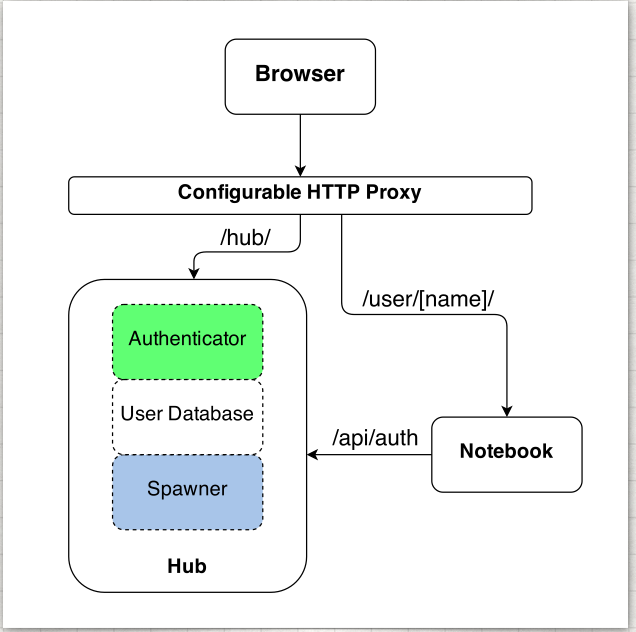
\includegraphics[width=0.52\textwidth]{images/jupyterhub_architecture.png}
\label{fig:jhub_architecture}
\end{figure}

This distinction is important for resource-aware notebook provisioning. The Hub does not itself perform user computations. Instead, the spawner translates the desired user environment into the configuration required by the underlying execution platform, creating and tearing down instances as users arrive and leave.

JupyterHub also provides an abstract Spawner interface for starting, polling, and stopping single-user notebook servers \cite{jupyterhub-spawners}. Different spawner implementations can use different execution backends, including local operating system processes, container runtimes, and Kubernetes clusters. In a Kubernetes deployment, KubeSpawner creates each user's notebook server as a dedicated Kubernetes workload \cite{kspawner,z2jh}. A spawner can also expose configuration options through the JupyterHub spawn form. Such options may represent CPU and memory allocations, container images, or a predefined combination of settings called a profile. JupyterHub's documentation explicitly describes profiles as a mechanism through which users can select a bundle of configuration settings for their notebook server \cite{jupyterhub-spawners}. A profile therefore provides an abstraction between low-level infrastructure configuration and user choice. Rather than requiring users to understand the exact Kubernetes resource specification, an administrator can define a small set of named environments such as \emph{Small}, \emph{Medium}, and \emph{Large}. The user then selects the environment that appears appropriate for the workload. However, manual selection often imposes substantial cognitive burden and decision difficulty on users who lack infrastructure expertise \cite{jameson}, underscoring the need for assistive decision-support mechanisms in complex choice environments \cite{parasuraman}. This mechanism provides an important foundation for automated environment recommendation. The recommendation problem can be formulated as selecting one of a finite set of administrator-defined environments rather than generating arbitrary infrastructure configurations dynamically.

\section{Kubernetes-based notebook execution}

\subsection{Containers and pods}

Kubernetes provides an orchestration layer for containerized applications. The basic execution unit relevant to a JupyterHub deployment is the Pod \cite{k8sresources}. A Pod contains one or more containers that share storage volumes, a network namespace with a single IP address, and specifications on how to run the workloads. Figure~\ref{fig:k8s_pod} illustrates the conceptual structure of a Pod encapsulating containerized components and shared storage. For notebook platforms, a user's single-user server is represented by a dedicated Pod where the container image determines the software environment available to the user, while the Kubernetes resource configuration determines the computational envelope allocated to the workload.

\begin{figure}[htbp]{Conceptual structure of a Kubernetes Pod encapsulating containers and shared storage volumes \cite{k8sresources}}
\centering
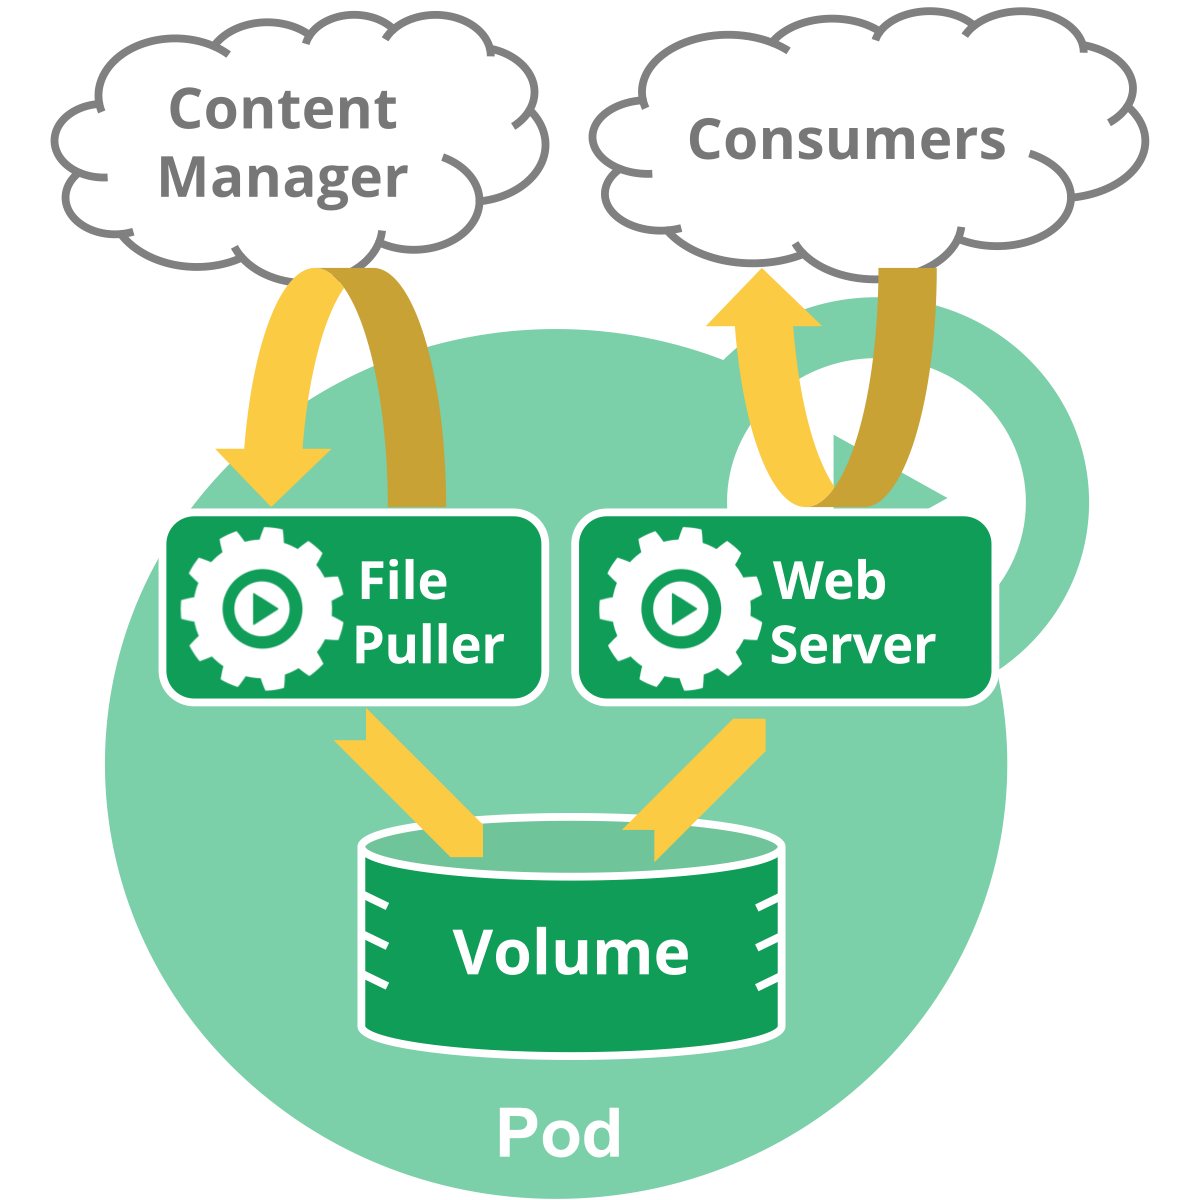
\includegraphics[width=0.48\textwidth]{images/kubernetes_pod.png}
\label{fig:k8s_pod}
\end{figure}

This separation establishes two complementary dimensions of environment selection. On the software dimension, the container image defines the runtime environment, pre-installed frameworks, domain-specific libraries, and underlying system dependencies. On the hardware resource dimension, the allocated CPU, memory, specialized hardware accelerators or GPUs \cite{k8sgpu}, and associated platform limits establish the computational envelope in which the workload executes. Consequently, an automated environment recommendation system must jointly consider both dimensions rather than treating resource sizing and software selection as unrelated choices.

\subsection{CPU and memory resources}

Kubernetes allows resource requests and limits to be specified for containers \cite{k8sresources}. A resource request represents the amount of a resource guaranteed and considered by the Kubernetes scheduler during node placement, while a resource limit establishes an upper bound on resource consumption enforced at runtime \cite{k8sscheduler}. For CPU and memory, these settings carry distinct operational implications. The Kubernetes scheduler uses resource requests when determining whether a Pod can be placed on a node without violating capacity constraints. In contrast, resource limits are enforced by kernel control groups: CPU limits can lead to CPU throttling when exceeded, whereas memory limits cause out-of-memory (OOM) terminations when memory pressure forces a container beyond its configured boundary \cite{k8sresources,k8sqos}. Furthermore, aggregate namespace allocations can be restricted using ResourceQuota objects \cite{k8squota}. Consequently, resource configuration must balance two competing operational concerns. If a profile provides too few resources, a workload may fail through OOM kills or suffer severe performance degradation. If it provides substantially more resources than necessary, the environment consumes cluster capacity that could otherwise serve other concurrent users, leading to widespread over-allocation and resource stranding observed in production multi-tenant clusters \cite{resourcecentral,autopilot,vpa}. For a multi-user notebook platform, resource-profile selection is thus a practical systems decision problem rather than merely a cosmetic interface preference.

\subsection{Resource profiles}

A resource profile is a predefined mapping from a human-readable environment choice to concrete infrastructure configurations. In the context of the proposed system, the repository defines three representative static profiles. The \emph{Small} profile is intended for basic Python programming and lightweight notebook workloads, offering modest resource allocations to maximize cluster density. The \emph{Medium} profile is configured for moderate data exploration, tabular data processing, and visualization tasks that require additional memory headroom. The \emph{Large} profile is designed for compute- and memory-intensive workloads, such as local model training or iterative numerical experimentation. The profiles differ systematically in their CPU and memory allocations. For example, the repository configuration defines the Small profile with a CPU guarantee of \(0.1\) cores, a CPU limit of \(0.5\) cores, a memory guarantee of \(256\)~MiB, and a memory limit of \(384\)~MiB. The Medium and Large profiles provide progressively larger resource envelopes. These values represent administrative policy choices rather than universal definitions of workload scale. Their primary role is to provide a finite, administrator- controlled candidate space from which a recommendation can be selected. This distinction is central to the system developed in this thesis. The recommendation component does not invent arbitrary CPU or memory values. Instead, it selects an environment from the administrator-defined catalog and verifies the selected candidate against explicit policy and capacity constraints.

\section{Notebook container images}

A container image packages the software environment required to execute a workload, encompassing the base operating system runtime, language interpreters, scientific libraries, machine-learning frameworks, and supporting system packages \cite{oci}. As shown in Figure~\ref{fig:container_layers}, container images follow a layered filesystem architecture where immutable, content-addressed read-only layers are stacked together, and a thin read-write layer is added at runtime when a container is instantiated \cite{dockerlayers}. This layered design enables efficient image distribution and local layer sharing across diverse notebook configurations, as empirical analyses of container workloads and image registries demonstrate significant redundancy and reuse potential across layer stacks \cite{anwar,harter}.

\begin{figure}[htbp]{Layered container image architecture with stacked read-only layers and a top read-write container layer \cite{dockerlayers}}
\centering
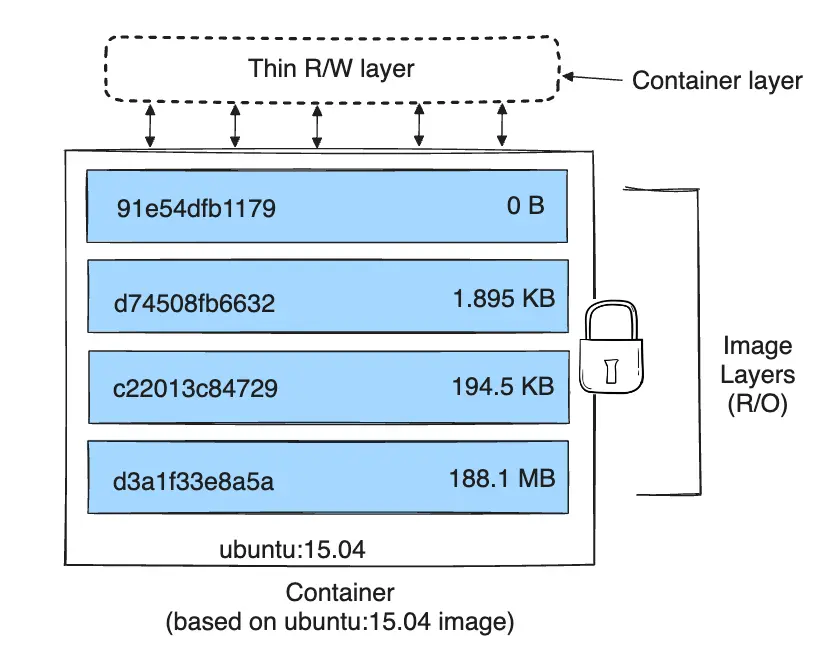
\includegraphics[width=0.52\textwidth]{images/container_layers.png}
\label{fig:container_layers}
\end{figure}

Different computational workloads inherently require different software stacks. A general programming task may require only a minimal Python runtime, while a data-analysis workflow requires packages such as NumPy, pandas, SciPy, and scikit-learn. Deep-learning workloads instead depend on specialized frameworks such as PyTorch or TensorFlow alongside accelerator drivers and CUDA runtime libraries. The proposed system models an execution environment as a coupled pair consisting of an approved resource profile and an administrator- reviewed notebook image, allowing the recommendation process to account simultaneously for computational resources and software dependencies.

Allowing an automated system to freely generate or pull arbitrary container image references introduces significant operational, security, and stability risks. An unvetted image may contain malicious code, outdated software, or incompatible dependencies that disrupt cluster operation. For this reason, the platform relies on an administrator-owned image catalog. The representative catalog entries include \texttt{minimal-python} for general Python programming and lightweight workloads, \texttt{scipy-data-science} for scientific computing, visualization, and conventional machine learning, \texttt{pytorch-deep-learning} for PyTorch-based deep-learning tasks, and \texttt{tensorflow-deep-learning} for TensorFlow- and Keras-based workflows. Each catalog entry is annotated with structured metadata detailing supported task types, frameworks, libraries, hardware capabilities, and suitability tags. This metadata provides a searchable semantic representation of the available environments, while also establishing an authoritative trust boundary: the recommendation algorithm is restricted to selecting among administrator-reviewed candidates rather than producing unverified container references.

\section{Workload intent}

Traditional resource-profile selection exposes infrastructure concepts directly to the end user. A user must determine whether a workload requires a small, medium, or large environment and separately identify which container image contains the appropriate software packages. This approach assumes that users can accurately translate their computational requirements into infrastructure specifications. In practice, users describe their goals in terms of the task they wish to perform. For example, a user may describe a workload as ``I want to train a PyTorch model on a large dataset.'' Such a description conveys information regarding the computational task, framework, and relative data scale, but it does not specify concrete Kubernetes CPU or memory allocations. The central abstraction used by the proposed system is therefore \emph{workload intent}, drawing on the principles of intent-based computing where high-level user goals are translated into system configurations \cite{rfc9315,leivadeas,wu}. Workload intent provides a structured representation of what the user wants to accomplish and what operational properties the resulting computational environment must satisfy.

Natural-language expressions provided by human users are inherently heterogeneous, unstructured, and ambiguous. A user describing a computational goal typically focuses on domain objectives (such as the machine learning framework, analytical procedure, or estimated dataset size) rather than low-level infrastructure attributes. Translating such unstructured natural-language requests into executable system configurations or platform commands is a recognized challenge in systems interfaces \cite{nl2bash}. Intent-based computing formalizes this paradigm by decoupling user intent specification from underlying execution configuration \cite{rfc9315,leivadeas}. Under this framework, high-level intent is translated into a validated, declarative contract that captures functional goals, explicit constraints, and user preferences. By establishing a structured intermediate representation, intent-based systems isolate the stochastic nature of natural language interpretation from deterministic execution engines. This structured bridge enables automated systems to parse user goals, validate semantic consistency, and apply rigorous policy enforcement without giving natural-language interfaces direct access to infrastructure provisioning mechanisms \cite{wu}.

\section{Information retrieval}\label{sec:ir_background}

The environment catalog used by the proposed system is a finite collection of administrator-defined computational environments. Each environment is associated with structured metadata describing properties such as supported workload types, frameworks, libraries, capabilities, and resource characteristics. The recommendation problem can therefore be viewed as a search problem over this catalog: given a user's workload description, the system must identify the environments whose metadata is most relevant to the request. This perspective motivates the use of \emph{information retrieval} (IR). Rather than requiring every possible natural-language expression to be explicitly encoded as a rule, retrieval allows the system to search the existing environment catalog and produce a ranked set of potentially relevant candidates.

Let
\[
    \mathcal{D} = \{d_1, d_2, \ldots, d_n\}
\]
represent the administrator-defined environment catalog and let \(q\) represent the user's workload intent. A retrieval function produces a ranked list
\[
    R(q) = (d_{(1)}, d_{(2)}, \ldots, d_{(k)}),
\]
where candidates appearing earlier in the list are considered more relevant to the query.

The use of retrieval is particularly appropriate because the system does not need to construct a new environment for every request. Instead, it searches within a controlled catalog and identifies candidates that already exist. This also preserves the administrator-defined boundary of the system: retrieval determines which existing environments are relevant, while subsequent constraint evaluation determines which of them are actually feasible. A straightforward approach would be to match the words in the user's request directly against the metadata of available environments. Although simple and interpretable, exact keyword matching is sensitive to differences in vocabulary. For example, a user may describe a workload as ``training a neural network'', while an environment may be described using terms such as ``deep learning'', ``PyTorch'', or ``model training''. These expressions may refer to related workloads without sharing exactly the same words. The opposite problem can also occur. Technical terms such as ``PyTorch'', ``TensorFlow'', or ``CUDA'' carry specific meanings and should not necessarily be treated as interchangeable with loosely related concepts. Consequently, an effective retrieval mechanism should provide both lexical precision for explicit technical terminology and tolerance to variations in natural-language expression. This motivates the use of two complementary retrieval approaches: sparse lexical retrieval and dense semantic retrieval.

\subsection{Sparse retrieval and BM25}\label{subsec:bm25_theory}

Sparse information retrieval methods represent queries and candidate documents primarily through their lexical features. They are particularly effective when important concepts are explicitly expressed using the same terms in the query and candidate metadata.

BM25 is a widely used probabilistic ranking function \cite{bm25}. Given a query \(Q\) and document \(D\), its score can be expressed as
\[
    \operatorname{BM25}(D,Q)
    =
    \sum_{t\in Q}
    \operatorname{IDF}(t)
    \cdot
    \frac{
        f(t,D)(k_1+1)
    }{
        f(t,D)+k_1
        \left(
            1-b+b\frac{|D|}{\operatorname{avgdl}}
        \right)
    },
\]
where \(f(t,D)\) is the frequency of term \(t\) in document \(D\), \(|D|\) is the document length, \(\operatorname{avgdl}\) is the average document length across the corpus, \(\operatorname{IDF}(t)\) is the inverse document frequency of term \(t\), and \(k_1\) and \(b\) control term-frequency saturation and length normalization, respectively. BM25 is useful for the proposed environment catalog because explicit technical vocabulary can be highly informative. For example, a request containing ``pandas'' can be matched directly against an environment whose metadata contains ``pandas''. Similarly, an explicit mention of ``PyTorch'' can provide strong evidence for a PyTorch-oriented environment. However, BM25 primarily relies on lexical overlap. If a user and an environment describe the same concept using substantially different vocabulary, their lexical similarity may be low. Therefore, BM25 alone does not fully address the variability of natural-language workload descriptions.

\subsection{Dense retrieval}\label{subsec:dense_theory}

Dense retrieval addresses vocabulary mismatch by representing queries and candidate environments as vectors in a continuous embedding space \cite{sentencebert,dpr,sparse_dense}. Let \(\mathbf{q} = f(q)\) be the embedding of a query and \(\mathbf{d} = f(d)\) be the embedding of a candidate environment. A common similarity measure is cosine similarity:
\[
    \operatorname{sim}(\mathbf{q},\mathbf{d})
    =
    \frac{\mathbf{q}\cdot\mathbf{d}}{\|\mathbf{q}\|\|\mathbf{d}\|}.
\]
Candidates with larger similarity values are considered semantically closer to the query.

The main advantage of dense retrieval is its ability to capture semantic relationships beyond exact word overlap. For example, a query describing ``neural-network training'' may be considered semantically related to an environment described as supporting ``deep learning'' and ``model training'', even if the two descriptions do not share all of their terms. Dense retrieval alone, however, also has limitations for this application. Embedding similarity may treat technically related expressions as similar even when an exact distinction is important. For example, different machine learning frameworks may be semantically related but are not necessarily interchangeable when a user explicitly requires one particular framework. The ranking produced by dense retrieval can also depend strongly on the embedding model and the representation of the candidate metadata. Therefore, dense retrieval is useful for discovering semantic relationships, but it should not be treated as the sole mechanism for interpreting explicit technical requirements.

\subsection{Hybrid retrieval with reciprocal rank fusion}\label{subsec:rrf_theory}

The characteristics of the environment recommendation problem suggest that neither sparse nor dense retrieval is sufficient on its own. Sparse retrieval provides strong lexical sensitivity. This is valuable when a user explicitly mentions technical entities such as a programming framework, library, or capability. Dense retrieval provides semantic flexibility and can help identify relevant environments when the user's wording differs from the wording used in the catalog. These properties are complementary. Sparse retrieval is effective for explicit terminology and exact technical concepts, dense retrieval is effective for semantic similarity and variation in natural-language descriptions, and hybrid retrieval combines these signals to obtain a broader candidate set while retaining sensitivity to explicit technical vocabulary. Hybrid retrieval is therefore selected as the retrieval strategy for the proposed system. The goal is not to allow semantic similarity to override explicit requirements, but to improve the identification of relevant candidates before deterministic constraint evaluation. This distinction is important. Retrieval is responsible for answering ``\emph{Which environments appear relevant to this workload?}'', whereas the subsequent constraint layer answers ``\emph{Which of these environments are actually allowed and feasible?}''. Separating these two questions prevents a high semantic similarity score from being treated as sufficient evidence that an environment satisfies a mandatory requirement.

Let \(r_s(d)\) and \(r_d(d)\) denote the ranks assigned to candidate \(d\) by the sparse and dense retrieval methods, respectively. Their rankings can be combined using Reciprocal Rank Fusion (RRF) \cite{rrf}:
\[
    \operatorname{RRF}(d)
    =
    \sum_{m\in\{s,d\}}
    \frac{w_m}{k_{\mathrm{RRF}}+r_m(d)},
\]
where \(w_m\) is the weight assigned to retrieval method \(m\), and \(k_{\mathrm{RRF}}\) is a constant controlling the contribution of lower-ranked candidates.

RRF is suitable for combining the two retrieval channels because it operates on rankings rather than requiring their raw scores to be directly comparable. This is useful in this setting because BM25 scores and embedding similarities have different numerical scales and interpretations. The resulting hybrid ranking provides the candidate set for the next stage of the recommendation pipeline. Importantly, this ranking is not itself the final provisioning decision. Retrieved candidates are subsequently evaluated against hard resource and software constraints and may then be ordered using soft preferences.

\section{Constraint-based recommendation}

Information retrieval assesses lexical and semantic relevance, but relevance alone is insufficient for decision-support and resource provisioning systems. A candidate solution may demonstrate high textual affinity to a user query while failing to meet mandatory operational requirements, physical prerequisites, or administrative policies. For domains governed by explicit rules, recommendation systems must incorporate constraint satisfaction mechanisms to guarantee solution validity. Constraint-based recommendation represents a major paradigm within knowledge-based recommender systems, designed for complex problem domains where items must satisfy strict technical specifications, compatibility rules, and domain constraints \cite{constraintrec}. Unlike collaborative filtering or pure content-based retrieval models that rely primarily on statistical correlation or historical usage patterns, constraint-based approaches model the recommendation task by combining constraint satisfaction with multi-attribute utility optimization.

In constraint-based recommendation theory, domain criteria are partitioned into two fundamental categories. Hard constraints are strict, non-negotiable operational requirements that define the boundary of valid solutions. A candidate item must satisfy all hard constraints simultaneously to be considered feasible. In technical systems, hard constraints prevent severe runtime failures (such as resource exhaustion or missing runtime dependencies), because violations cannot be compensated for or traded off against high relevance scores. On the other hand, soft constraints and preferences are desirable but optional criteria that express user affinities, quality indicators, or secondary optimization goals. Soft preferences are evaluated across the set of verified feasible solutions using multi-attribute utility functions, guiding the ranking of viable candidates without compromising feasibility \cite{herlocker,jarvelin}. Furthermore, evaluating such decision-support systems requires examining not only algorithmic accuracy but also user perception, trust, and decision quality, as established in user-centric recommender system evaluation frameworks \cite{pu,knijnenburg}. Structuring the decision-support pipeline into a two-phase architecture candidate retrieval followed by deterministic constraint evaluation and utility ranking ensures both search efficiency and operational correctness. Candidate retrieval efficiently narrows a large catalog down to a promising subset, while subsequent constraint filtering guarantees that only viable, policy-compliant candidates proceed to final ranking and deployment.